\section{Multicore}
\subsection{Steigern der Geschwindigkeit eines Prozessors}
Die Geschwindigkeit eines Prozessors kann mit den folgenden Methoden gesteigert werden.

\subsubsection{Clockfrequenz erhöhen}
\begin{itemize}
	\item PCB-Design wird sehr anspruchsvoll  (Leitungslängen, Reflexionen, etc.)
	\item Elektrische Verlustleistung steigt linear mit der Clockfrequenz (Hitzeproblematik)
	\begin{equation}
		P = f_{cl} \cdot C_L \cdot V_{dd}^2
	\end{equation}
	\item Lichtgeschwindigkeit ist die Grenze.
\end{itemize}

\subsubsection{Instruction-level parallelism (ILP)}
\begin{itemize}
	\item Parallelismus wird auf Instruktionslevel angestrebt 
	\begin{itemize}
		\item Pipelines
		\item Verschachteln der Instruktionen, um Pipeline möglichst optimal auszulasten 
		\item Vermeiden von Pipeline flush durch Vorhersage der Verzweigung (branch prediction) 
	\end{itemize}
	\item Branch prediction kann sehr aufwendig werden 
	\item Compiler werden komplex
\end{itemize}

\begin{multicols}{2}
\subsubsection{Thread-level parallelism (TLP)}
\begin{itemize}
	\item Parallelisiert wird auf einer umfangreicheren Stufe als nur auf der Instruktion 
	\item Die parallelisierte Einheit ist in der Grössenordnung einer Funktion 
	\item Zugriffe auf gemeinsame Ressourcen, z.B. sharedmemory, müssen geregelt werden 
	\item Design Issues 
	\begin{itemize}
		\item Nicht einfach beliebig viele Threads spendieren 
		\item Jeder Thread erzeugt Overhead 
		\item Die Threads sollten möglichst unabhängig voneinander sein
		\item Wenn zu viele Threads definiert werden (wenn Zusammengehörendes auseinandergenommen wird), dann werden Daten unnötigerweise shared
	\end{itemize}		
\end{itemize}
\columnbreak
\paragraph{Umsetzung}
\begin{itemize}
	\item Uniprocessor(single-core) 
	\begin{itemize}
		\item Die Threads werden time-sliced 
		\item Pseudo-TLP
		\item Context switch notwendig
	\end{itemize}
	\item  Multiprocessor(Computer mit mehreren Prozessoren) 
	\begin{itemize}
		\item Mehrere parallele Prozessoren können je einen Thread bearbeiten 
		\item Echter TLP 
		\item Clockfrequenzkann tiefer gehalten werden 
		\item Einfachere Hardware wird multipliziert 
		\item Datenaustausch zwischen Prozessoren muss irgendwie geregelt werden, z.B. mit Message Passing oder SharedMemory
	\end{itemize}
\end{itemize}
\end{multicols}

\subsection{Multicore Prozessor}
\begin{multicols}{2}
	\begin{itemize}
		\item Ein Multicore Prozessor ist ein spezieller Multiprocessor. Alle Prozessoren (Cores) befinden sich auf demselben Chip
		\item  Multicore Prozessoren sind MIMD (Multiple Instructions Multiple Data). Jeder Core führt einen eigenen Code aus und arbeitet auf unterschiedlichen Daten 
		\item Die Speicherorganisation ist oft komplex
		\item Zwei Typen
		\begin{itemize}
			\item Homogener Multicore Prozessor (mehrere gleiche Cores)
			\item Heterogener Multicore Prozessor (mehrere gleiche/unterschiedliche Cores). Häufig bei Embedded Multicore Prozessoren		
		\end{itemize}
	\end{itemize}
\columnbreak
	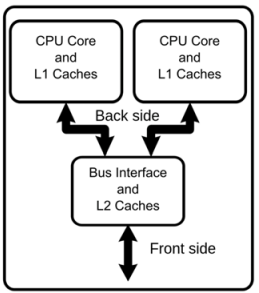
\includegraphics[width=0.4\textwidth]{images/Multicore/Multicore}
\end{multicols}

\subsubsection{Amdahl's Law}
Gesamtaufgabe soll auf möglichst viele Cores aufgeteilt werden, um eine optimale Ausführungszeit zu erzielen. \\
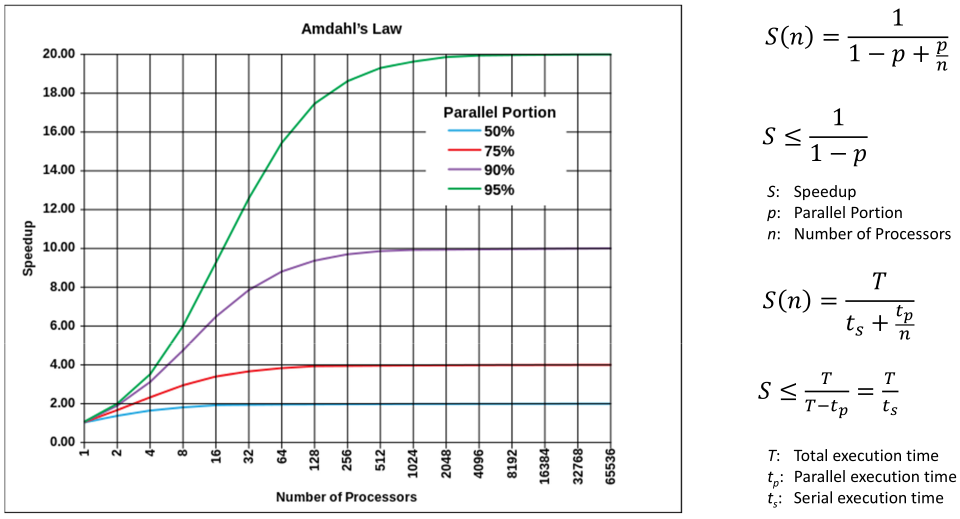
\includegraphics[width=1\textwidth]{images/Multicore/amdahl}

\subsubsection{Speicherorganisation}
\begin{multicols}{2}
	\begin{itemize}
		\item Shared Memory
		\begin{itemize}
			\item Alle Prozessoren nutzen einen gemeinsamen Speicherbereich 
			\item Einfache Implementation 
			\item Shared Memory kann zum Flaschenhals werden 
		\end{itemize}
	\end{itemize}
\columnbreak
	\begin{itemize}
		\item Distributed Memory
		\begin{itemize}
			\item Jeder Prozessor hat seinen eigenen lokalen Speicher 
			\item Für den Datenaustausch unter den Prozessoren muss wiederum ein Mechanismus zur Verfügung gestellt werden, z.B. Message Passing
		\end{itemize}
	\end{itemize}
\end{multicols}

